\section{Preliminary Case Study}
\subsection{Setup}
\begin{frame}
    \Huge{\centerline{\textbf{Preliminary Case Study}}}
\end{frame}

\subsection{Aralia Fault Tree Data Set}
\begin{frame}[t]
\frametitle{Overview: Aralia Dataset}
\begin{itemize}
  \item \textbf{Dataset Composition:} The Aralia collection consists of 43 distinct fault trees, each with varying numbers of basic events (BEs), gate types (AND, OR, K/N, XOR), and minimal cut-set counts.  
  \item \textbf{Diverse Problem Sizes:} Small trees (e.g.\ 25--32 BEs) through large models with over 1{,}500 BEs.  
  \item \textbf{Wide Probability Range:} Top-event probabilities spanning from rare events near \(10^{-13}\) to fairly likely failures with probability above 0.7.  
  \item \textbf{Model Variability:} Some trees are primarily AND/OR, others incorporate more advanced gates (K/N, XOR, NOT), providing thorough coverage of typical (and atypical) fault tree logic structures.
\end{itemize}
\end{frame}

\begin{frame}[allowframebreaks]
    

% Please add the following required packages to your document preamble:
% \usepackage{booktabs}
% \usepackage{multirow}
% \usepackage[table,xcdraw]{xcolor}
% Beamer presentation requires \usepackage{colortbl} instead of \usepackage[table,xcdraw]{xcolor}
% \usepackage{longtable}
% Note: It may be necessary to compile the document several times to get a multi-page table to line up properly
\tiny
\begin{longtable}{@{}llrrrrrrrc@{}}
\label{tab:my-table}\\
\toprule
            &          & \multicolumn{1}{c}{} & \multicolumn{5}{c}{\textbf{Logic Gates}} & \multicolumn{1}{c}{} &             \\* \cmidrule(lr){4-8}
\multirow{-2}{*}{\textbf{\#}} &
  \multirow{-2}{*}{\textbf{\begin{tabular}[c]{@{}l@{}}Fault\\ Tree\end{tabular}}} &
  \multicolumn{1}{c}{\multirow{-2}{*}{\textbf{\begin{tabular}[c]{@{}c@{}}Basic\\ Events\end{tabular}}}} &
  \multicolumn{1}{c}{\textbf{Total}} &
  \multicolumn{1}{c}{AND} &
  \multicolumn{1}{c}{K/N} &
  \multicolumn{1}{c}{XOR} &
  \multicolumn{1}{c}{NOT} &
  \multicolumn{1}{c}{\multirow{-2}{*}{\textbf{\begin{tabular}[c]{@{}c@{}}Minimal\\ Cut Sets\end{tabular}}}} &
  \multirow{-2}{*}{\textbf{\begin{tabular}[c]{@{}c@{}}Top Event\\ Probability\end{tabular}}} \\* \midrule
\endhead
%
\bottomrule
\endfoot
%
\endlastfoot
%
\textbf{1}  & baobab1  & 61                   & 84       & 16      & 9    & -    & -     & 46,188               & 1.01708E-04 \\
\textbf{2}  & baobab2  & 32                   & 40       & 5       & 6    & -    & -     & 4,805                & 7.13018E-04 \\
\textbf{3}  & baobab3  & 80                   & 107      & 46      & -    & -    & -     & 24,386               & 2.24117E-03 \\
\textbf{4}  & cea9601  & 186                  & 201      & 69      & 8    & -    & 30    & 130,281,976          & 1.48409E-03 \\
\textbf{5}  & chinese  & 25                   & 36       & 13      & -    & -    & -     & 392                  & 1.17058E-03 \\
\textbf{6}  & das9201  & 122                  & 82       & 19      & -    & -    & -     & 14,217               & 1.34237E-02 \\
\textbf{7}  & das9202  & 49                   & 36       & 10      & -    & -    & -     & 27,778               & 1.01154E-02 \\
\textbf{8}  & das9203  & 51                   & 30       & 1       & -    & -    & -     & 16,200               & 1.34880E-03 \\
\textbf{9}  & das9204  & 53                   & 30       & 12      & -    & -    & -     & 16,704               & 6.07651E-08 \\
\textbf{10} & das9205  & 51                   & 20       & 2       & -    & -    & -     & 17,280               & 1.38408E-08 \\
\textbf{11} & das9206  & 121                  & 112      & 21      & -    & -    & -     & 19,518               & 2.29687E-01 \\
\textbf{12} & das9207  & 276                  & 324      & 59      & -    & -    & -     & 25,988               & 3.46696E-01 \\
\textbf{13} & das9208  & 103                  & 145      & 33      & -    & -    & -     & 8,060                & 1.30179E-02 \\
\textbf{14} & das9209  & 109                  & 73       & 18      & -    & -    & -     & 8.20E+10             & 1.05800E-13 \\
\textbf{15} & das9601  & 122                  & 288      & 60      & 36   & 12   & 14    & 4,259                & 4.23440E-03 \\
\textbf{16} & das9701  & 267                  & 2,226    & 1,739   & -    & -    & 992   & 26,299,506           & 7.44694E-02 \\
\textbf{17} & edf9201  & 183                  & 132      & 12      & -    & -    & -     & 579,720              & 3.24591E-01 \\
\textbf{18} & edf9202  & 458                  & 435      & 45      & -    & -    & -     & 130,112              & 7.81302E-01 \\
\textbf{19} & edf9203  & 362                  & 475      & 117     & -    & -    & -     & 20,807,446           & 5.99589E-01 \\
\textbf{20} & edf9204  & 323                  & 375      & 106     & -    & -    & -     & 32,580,630           & 5.25374E-01 \\
\textbf{21} & edf9205  & 165                  & 142      & 30      & -    & -    & -     & 21,308               & 2.09351E-01 \\
\textbf{22} & edf9206  & 240                  & 362      & 126     & -    & -    & -     & 385,825,320          & 8.61500E-12 \\
\textbf{23} & edfpa14b & 311                  & 290      & 70      & -    & -    & -     & 105,955,422          & 2.95620E-01 \\
\textbf{24} & edfpa14o & 311                  & 173      & 42      & -    & -    & -     & 105,927,244          & 2.97057E-01 \\
\textbf{25} & edfpa14p & 124                  & 101      & 42      & -    & -    & -     & 415,500              & 8.07059E-02 \\
\textbf{26} & edfpa14q & 311                  & 194      & 55      & -    & -    & -     & 105,950,670          & 2.95905E-01 \\
\textbf{27} & edfpa14r & 106                  & 132      & 55      & -    & -    & -     & 380,412              & 2.09977E-02 \\
\textbf{28} & edfpa15b & 283                  & 249      & 61      & -    & -    & -     & 2,910,473            & 3.62737E-01 \\
\textbf{29} & edfpa15o & 283                  & 138      & 33      & -    & -    & -     & 2,906,753            & 3.62956E-01 \\
\textbf{30} & edfpa15p & 276                  & 324      & 33      & -    & -    & -     & 27,870               & 7.36302E-02 \\
\textbf{31} & edfpa15q & 283                  & 158      & 45      & -    & -    & -     & 2,910,473            & 3.62737E-01 \\
\textbf{32} & edfpa15r & 88                   & 110      & 45      & -    & -    & -     & 26,549               & 1.89750E-02 \\
\textbf{33} & elf9601  & 145                  & 242      & 97      & -    & -    & -     & 151,348              & 9.66291E-02 \\
\textbf{34} & ftr10    & 175                  & 94       & 26      & -    & -    & -     & 305                  & 4.48677E-01 \\
\textbf{35} & isp9601  & 143                  & 104      & 25      & 1    & -    & -     & 276,785              & 5.71245E-02 \\
\textbf{36} & isp9602  & 116                  & 122      & 26      & -    & -    & -     & 5,197,647            & 1.72447E-02 \\
\textbf{37} & isp9603  & 91                   & 95       & 37      & -    & -    & -     & 3,434                & 3.23326E-03 \\
\textbf{38} & isp9604  & 215                  & 132      & 38      & -    & -    & -     & 746,574              & 1.42751E-01 \\
\textbf{39} & isp9605  & 32                   & 40       & 8       & 6    & -    & -     & 5,630                & 1.37171E-05 \\
\textbf{40} & isp9606  & 89                   & 41       & 14      & -    & -    & -     & 1,776                & 5.43174E-02 \\
\textbf{41} & isp9607  & 74                   & 65       & 23      & -    & -    & -     & 150,436              & 9.49510E-07 \\
\textbf{42} & jbd9601  & 533                  & 315      & 71      & -    & -    & -     & 150,436              & 7.55091E-01 \\
\rowcolor[HTML]{F2F2F2} 
\textbf{43} & nus9601  & 1,567                & 1,622    & 392     & 47   & -    & -     & unknown              & unknown     \\* \bottomrule
\end{longtable}
\end{frame}

\subsection{Benchmarking Procedure}
\begin{frame}[t]
\frametitle{Benchmarking Setup: Hardware and Environment}
\begin{itemize}
  \item \textbf{Target Hardware:}
    \begin{itemize}
      \item GPU: NVIDIA\textsuperscript{\textregistered} GeForce GTX 1660 SUPER (6\,GB GDDR6, 1{,}408 CUDA cores).
      \item CPU: Intel\textsuperscript{\textregistered} Core\textsuperscript{TM} i7-10700 (2.90\,GHz, turbo-boost, hyperthreading).
    \end{itemize}
  \item \textbf{Software Stack:}
    \begin{itemize}
      \item SYCL-based (AdaptiveCpp/HipSYCL), with LLVM-IR JIT for kernel compilation.
      \item Compiler optimization at \texttt{-O3} for efficient code generation.
      \item Repeated runs (5+) to mitigate transient variations.
    \end{itemize}
  \item \textbf{Measured Time:} Includes entire wall-clock duration, from host-device transfers and JIT compilation to final result collection.
\end{itemize}
\end{frame}

\begin{frame}[t]
\frametitle{Monte Carlo Execution and Implementation}
\begin{itemize}
  \item \textbf{Sampling Strategy:}
    \begin{itemize}
      \item Single pass per fault tree, generating as many samples as fit in 6\,GB GPU memory.  
      \item 128-bit Philox4x32x10 pseudo-random number generator, parallel threads.
    \end{itemize}
  \item \textbf{Bit-Packing Optimization:}
    \begin{itemize}
      \item Each group of 64 Monte Carlo outcomes stored in a single 64-bit word.  
      \item Enables vectorized instructions (e.g.\ \texttt{popcount}) and reduces memory I/O.
    \end{itemize}
  \item \textbf{Data Types:}
    \begin{itemize}
      \item Tallies in 64-bit integers.  
      \item Probability accumulations in double precision (64-bit float).  
    \end{itemize}
\end{itemize}
\end{frame}

\begin{frame}[allowframebreaks]
    \begin{figure}[h]
    \centering
    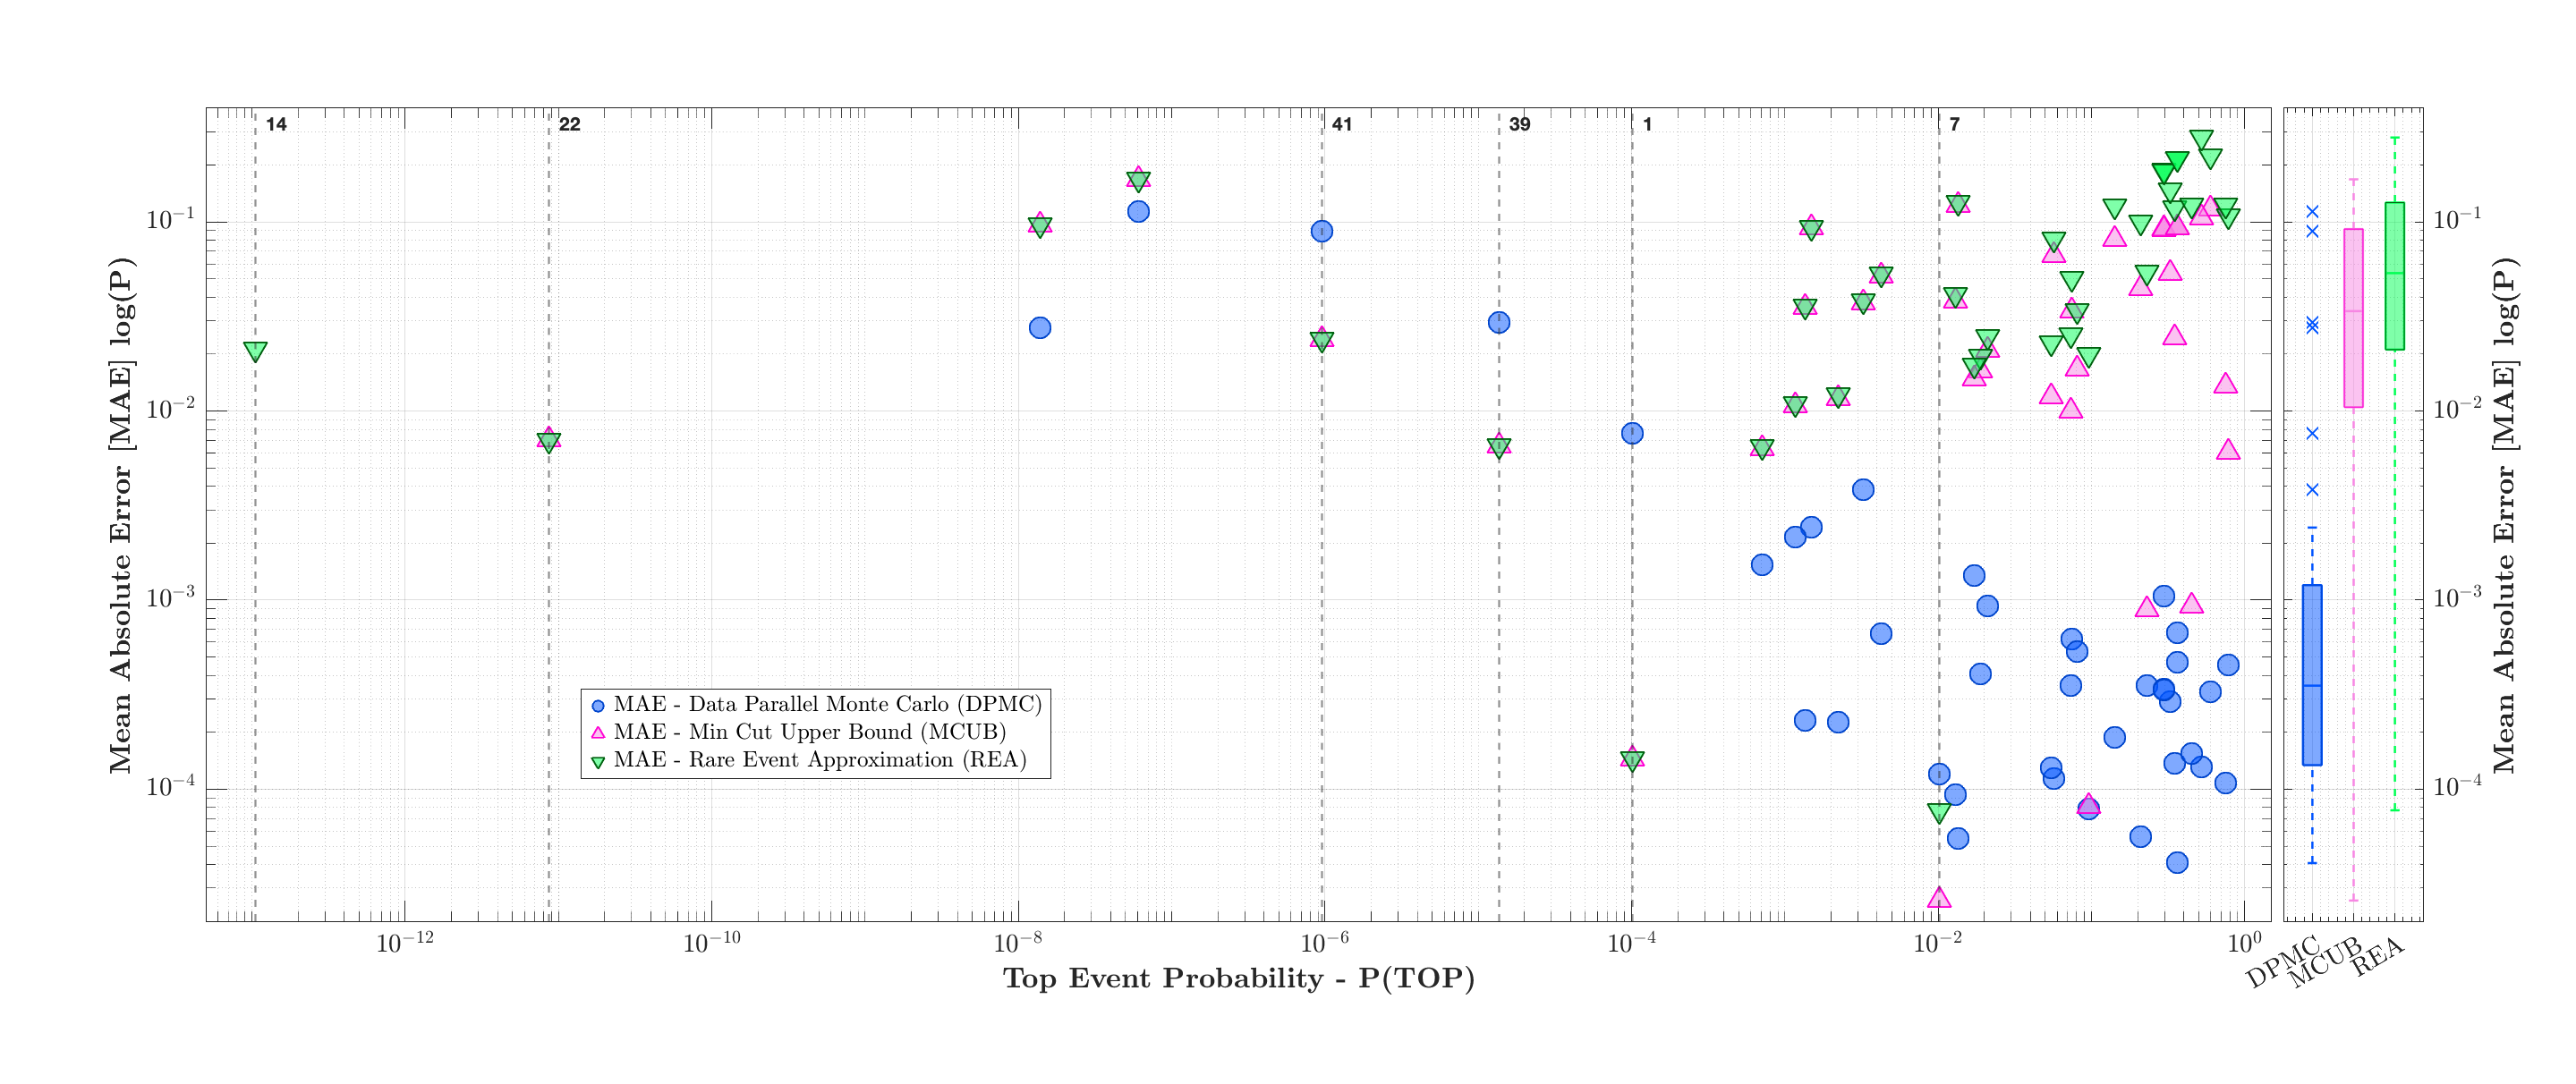
\includegraphics[width=0.9\textwidth]{4_casestudy/error_vs_prob_detailed.png}
    \caption{Mean Absolute Error – Exact (BDD) vs Approximate Methods}
    \label{fig:mae_vs_logp}
\end{figure}
\end{frame}

\begin{frame}[allowframebreaks]
    \begin{figure}[h]
    \centering
    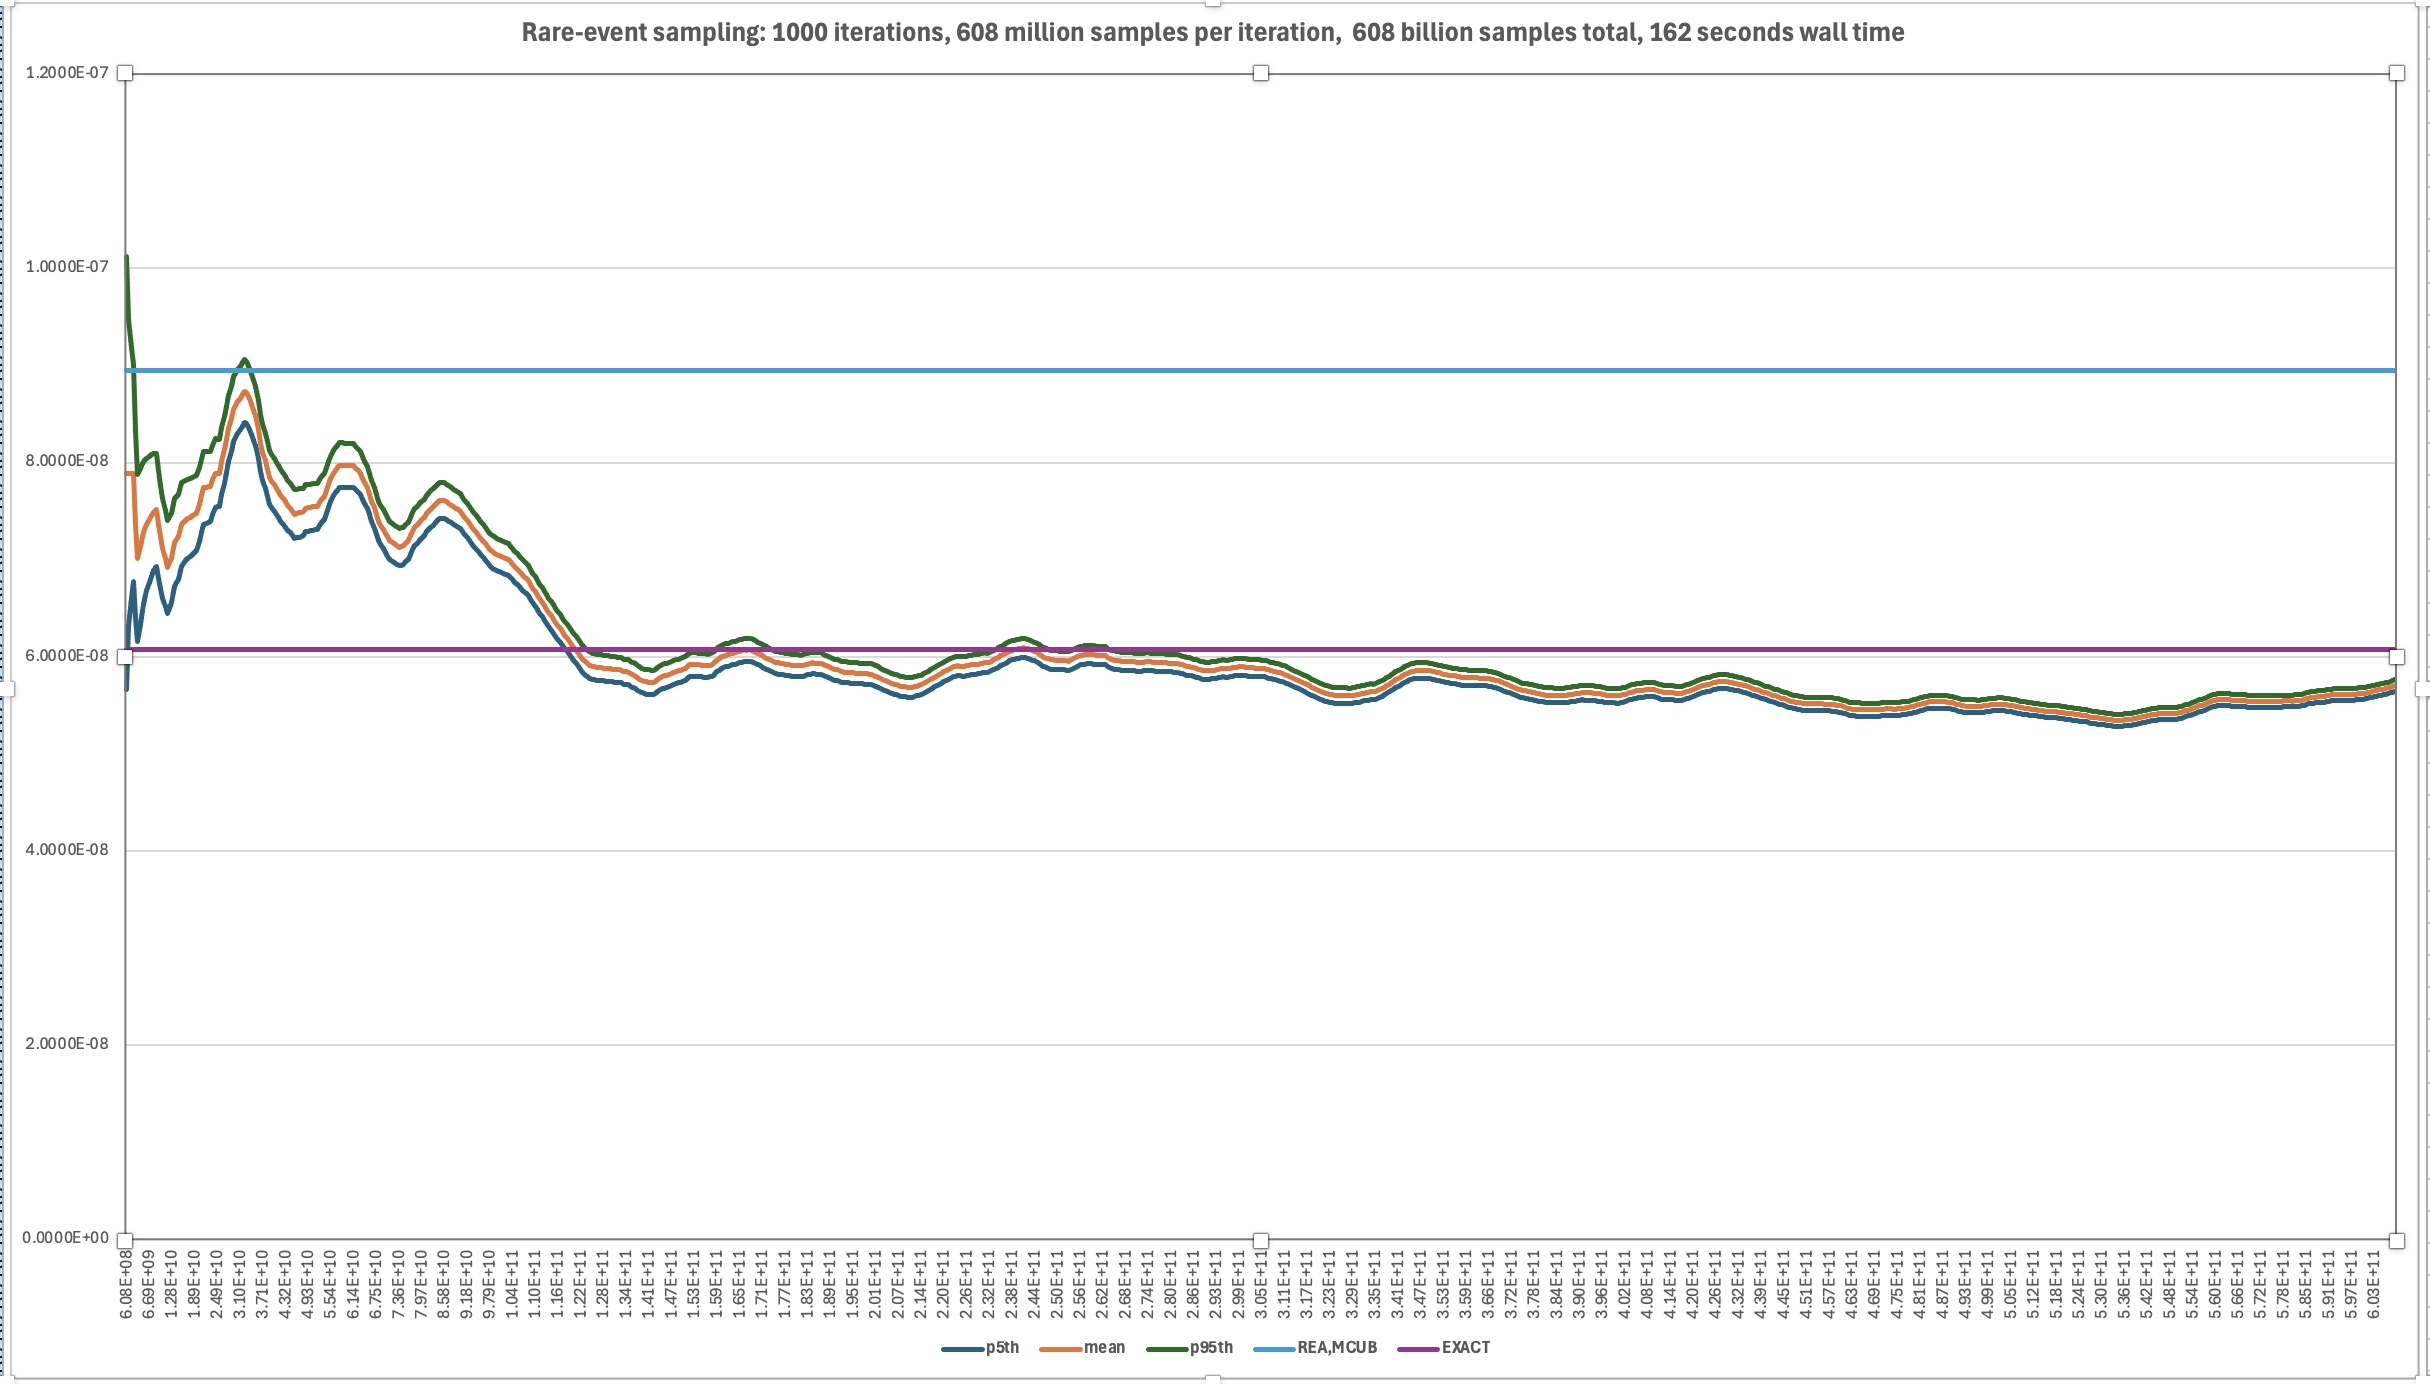
\includegraphics[width=0.7\textwidth]{4_casestudy/rare-event.jpg}
    \label{fig:rare}
\end{figure}
\end{frame}


\subsection{Aralia Fault Tree Data Set - Convergence for Rare Events}
\begin{frame}[allowframebreaks]
    \tiny
\sisetup{table-format=1.2e-2}
\begin{longtable}{@{}llS[table-format=1.2e-2]S[table-format=1.2e-2]S[table-format=1.2e-2]S[table-format=1.2e-2]l@{}}
\label{tab:logp-mae}\\
\toprule
            &          & \multicolumn{3}{c}{\textbf{Mean Absolute Error - log(P)}}       &         &       \\* \cmidrule(lr){3-5}
\multirow{-2}{*}{\textbf{\#}} &
  \multirow{-2}{*}{\textbf{\begin{tabular}[c]{@{}l@{}}Fault\\ Tree\end{tabular}}} &
  \textbf{REA} &
  \textbf{MCUB} &
  \cellcolor[HTML]{F2F2F2}\textbf{Monte Carlo} &
  \multirow{-2}{*}{\textbf{\begin{tabular}[c]{@{}l@{}}MC\\ Samples\end{tabular}}} &
  \multirow{-2}{*}{\textbf{\begin{tabular}[c]{@{}l@{}}Runtime\\ {[}sec{]}\end{tabular}}} \\* \midrule
\endhead
%
\bottomrule
\endfoot
%
\endlastfoot
%
\rowcolor[HTML]{E5E5E5} 
\textbf{1}  & baobab1  & 1.45156E-04 & 1.45156E-04 & 7.61880E-03                         & 2.5E+08 & 0.262 \\
\textbf{2}  & baobab2  & 6.48628E-03 & 6.34705E-03 & \cellcolor[HTML]{F2F2F2}1.54436E-03 & 2.5E+08 & 0.209 \\
\textbf{3}  & baobab3  & 1.21509E-02 & 1.16701E-02 & \cellcolor[HTML]{F2F2F2}2.24843E-04 & 2.4E+08 & 0.259 \\
\textbf{4}  & cea9601  & 9.36195E-02 & 9.32207E-02 & \cellcolor[HTML]{F2F2F2}2.41802E-03 & 1.2E+08 & 0.262 \\
\textbf{5}  & chinese  & 1.08742E-02 & 1.06354E-02 & \cellcolor[HTML]{F2F2F2}2.14601E-03 & 9.4E+08 & 0.277 \\
\textbf{6}  & das9201  & 1.26649E-01 & 1.22765E-01 & \cellcolor[HTML]{F2F2F2}5.49963E-05 & 2.3E+08 & 0.279 \\
\rowcolor[HTML]{E5E5E5} 
\textbf{7}  & das9202  & 7.72743E-05 & 2.57596E-05 & 1.20232E-04                         & 5.2E+08 & 0.295 \\
\textbf{8}  & das9203  & 3.59019E-02 & 3.55935E-02 & \cellcolor[HTML]{F2F2F2}2.31768E-04 & 5.2E+08 & 0.292 \\
\textbf{9}  & das9204  & 1.68086E-01 & 1.68087E-01 & \cellcolor[HTML]{F2F2F2}1.13495E-01 & 6.1E+08 & 0.292 \\
\textbf{10} & das9205  & 9.63825E-02 & 9.63725E-02 & \cellcolor[HTML]{F2F2F2}2.76190E-02 & 3.3E+09 & 0.958 \\
\textbf{11} & das9206  & 5.43561E-02 & 8.89660E-04 & \cellcolor[HTML]{F2F2F2}3.51548E-04 & 2.0E+08 & 0.269 \\
\textbf{12} & das9207  & 1.18486E-01 & 2.45492E-02 & \cellcolor[HTML]{F2F2F2}1.36519E-04 & 9.5E+07 & 0.282 \\
\textbf{13} & das9208  & 4.12808E-02 & 3.81968E-02 & \cellcolor[HTML]{F2F2F2}9.34017E-05 & 2.5E+08 & 0.307 \\
\rowcolor[HTML]{E5E5E5} 
\textbf{14} &
  das9209 &
  2.11242E-02 &
  1.70245E+01 &
   &
  \multicolumn{1}{c}{\cellcolor[HTML]{E5E5E5}-} &
  \multicolumn{1}{c}{\cellcolor[HTML]{E5E5E5}-} \\
\textbf{15} & das9601  & 5.29285E-02 & 5.19122E-02 & \cellcolor[HTML]{F2F2F2}6.67174E-04 & 1.1E+08 & 0.256 \\
\textbf{16} & das9701  & 5.02804E-02 & 3.37565E-02 & \cellcolor[HTML]{F2F2F2}6.22978E-04 & 2.3E+07 & 0.273 \\
\textbf{17} & edf9201  & 1.48012E-01 & 5.36182E-02 & \cellcolor[HTML]{F2F2F2}2.88906E-04 & 1.8E+08 & 0.315 \\
\textbf{18} & edf9202  & 1.07181E-01 & 6.05976E-03 & \cellcolor[HTML]{F2F2F2}4.53900E-04 & 7.8E+07 & 0.271 \\
\textbf{19} & edf9203  & 2.22146E-01 & 1.17293E-01 & \cellcolor[HTML]{F2F2F2}3.27993E-04 & 8.0E+07 & 0.302 \\
\textbf{20} & edf9204  & 2.79531E-01 & 1.05591E-01 & \cellcolor[HTML]{F2F2F2}1.31416E-04 & 8.7E+07 & 0.298 \\
\textbf{21} & edf9205  & 9.94339E-02 & 4.46260E-02 & \cellcolor[HTML]{F2F2F2}5.60146E-05 & 1.9E+08 & 0.284 \\
\rowcolor[HTML]{E5E5E5} 
\textbf{22} & edf9206  & 6.98797E-03 & 7.07775E-03 & -                                   & -       & -     \\
\textbf{23} & edfpa14b & 1.85574E-01 & 9.15983E-02 & \cellcolor[HTML]{F2F2F2}1.04767E-03 & 9.4E+07 & 0.267 \\
\textbf{24} & edfpa14o & 1.86482E-01 & 9.18665E-02 & \cellcolor[HTML]{F2F2F2}3.39049E-04 & 9.8E+07 & 0.275 \\
\textbf{25} & edfpa14p & 3.40010E-02 & 1.66283E-02 & \cellcolor[HTML]{F2F2F2}5.35099E-04 & 2.1E+08 & 0.294 \\
\textbf{26} & edfpa14q & 1.85609E-01 & 9.15366E-02 & \cellcolor[HTML]{F2F2F2}3.33292E-04 & 9.6E+07 & 0.282 \\
\textbf{27} & edfpa14r & 2.48088E-02 & 2.09729E-02 & \cellcolor[HTML]{F2F2F2}9.33865E-04 & 2.1E+08 & 0.294 \\
\textbf{28} & edfpa15b & 2.16329E-01 & 9.37065E-02 & \cellcolor[HTML]{F2F2F2}4.67881E-04 & 1.1E+08 & 0.283 \\
\textbf{29} & edfpa15o & 2.16502E-01 & 9.37627E-02 & \cellcolor[HTML]{F2F2F2}4.06846E-05 & 1.1E+08 & 0.282 \\
\textbf{30} & edfpa15p & 2.52568E-02 & 1.00382E-02 & \cellcolor[HTML]{F2F2F2}3.54344E-04 & 2.6E+08 & 0.299 \\
\textbf{31} & edfpa15q & 2.16329E-01 & 9.37065E-02 & \cellcolor[HTML]{F2F2F2}6.74736E-04 & 1.1E+08 & 0.284 \\
\textbf{32} & edfpa15r & 1.94693E-02 & 1.62668E-02 & \cellcolor[HTML]{F2F2F2}4.04924E-04 & 2.5E+08 & 0.290 \\
\textbf{33} & elf9601  & 1.98107E-02 & 8.08925E-05 & \cellcolor[HTML]{F2F2F2}7.86600E-05 & 2.3E+08 & 0.274 \\
\textbf{34} & ftr10    & 1.22076E-01 & 9.27268E-04 & \cellcolor[HTML]{F2F2F2}1.54844E-04 & 2.1E+08 & 0.297 \\
\textbf{35} & isp9601  & 8.08392E-02 & 6.63074E-02 & \cellcolor[HTML]{F2F2F2}1.13264E-04 & 1.8E+08 & 0.271 \\
\textbf{36} & isp9602  & 1.74572E-02 & 1.47782E-02 & \cellcolor[HTML]{F2F2F2}1.35280E-03 & 2.3E+08 & 0.281 \\
\textbf{37} & isp9603  & 3.82337E-02 & 3.74815E-02 & \cellcolor[HTML]{F2F2F2}3.82344E-03 & 2.7E+08 & 0.278 \\
\textbf{38} & isp9604  & 1.20889E-01 & 8.14313E-02 & \cellcolor[HTML]{F2F2F2}1.88665E-04 & 1.4E+08 & 0.280 \\
\rowcolor[HTML]{E5E5E5} 
\textbf{39} & isp9605  & 6.57344E-03 & 6.57032E-03 & 2.93472E-02                         & 5.0E+08 & 0.262 \\
\textbf{40} & isp9606  & 2.27811E-02 & 1.18983E-02 & \cellcolor[HTML]{F2F2F2}1.30307E-04 & 3.4E+08 & 0.289 \\
\rowcolor[HTML]{E5E5E5} 
\textbf{41} & isp9607  & 2.38880E-02 & 2.38880E-02 & 1.28136E-01                         & 3.8E+08 & 0.282 \\
\textbf{42} & jbd9601  & 1.22001E-01 & 1.35343E-02 & \cellcolor[HTML]{F2F2F2}1.08116E-04 & 5.7E+07 & 0.279 \\
\rowcolor[HTML]{DDDDDD} 
\textbf{43} & nus9601  &            & -           & -                                   & 1.6E+07 & 0.289 \\* \bottomrule
\end{longtable}
\end{frame}


% \begin{frame}{Aralia Fault Tree Dataset}
% show the input dataset table\\
% \end{frame}

% \subsection{Results}
% \begin{frame}{Mar}
% show the input dataset table\\
% \end{frame}